\documentclass[11pt, a4paper]{article}\usepackage[]{graphicx}\usepackage[]{xcolor}
% maxwidth is the original width if it is less than linewidth
% otherwise use linewidth (to make sure the graphics do not exceed the margin)
\makeatletter
\def\maxwidth{ %
  \ifdim\Gin@nat@width>\linewidth
    \linewidth
  \else
    \Gin@nat@width
  \fi
}
\makeatother

\definecolor{fgcolor}{rgb}{0.345, 0.345, 0.345}
\newcommand{\hlnum}[1]{\textcolor[rgb]{0.686,0.059,0.569}{#1}}%
\newcommand{\hlstr}[1]{\textcolor[rgb]{0.192,0.494,0.8}{#1}}%
\newcommand{\hlcom}[1]{\textcolor[rgb]{0.678,0.584,0.686}{\textit{#1}}}%
\newcommand{\hlopt}[1]{\textcolor[rgb]{0,0,0}{#1}}%
\newcommand{\hlstd}[1]{\textcolor[rgb]{0.345,0.345,0.345}{#1}}%
\newcommand{\hlkwa}[1]{\textcolor[rgb]{0.161,0.373,0.58}{\textbf{#1}}}%
\newcommand{\hlkwb}[1]{\textcolor[rgb]{0.69,0.353,0.396}{#1}}%
\newcommand{\hlkwc}[1]{\textcolor[rgb]{0.333,0.667,0.333}{#1}}%
\newcommand{\hlkwd}[1]{\textcolor[rgb]{0.737,0.353,0.396}{\textbf{#1}}}%
\let\hlipl\hlkwb

\usepackage{framed}
\makeatletter
\newenvironment{kframe}{%
 \def\at@end@of@kframe{}%
 \ifinner\ifhmode%
  \def\at@end@of@kframe{\end{minipage}}%
  \begin{minipage}{\columnwidth}%
 \fi\fi%
 \def\FrameCommand##1{\hskip\@totalleftmargin \hskip-\fboxsep
 \colorbox{shadecolor}{##1}\hskip-\fboxsep
     % There is no \\@totalrightmargin, so:
     \hskip-\linewidth \hskip-\@totalleftmargin \hskip\columnwidth}%
 \MakeFramed {\advance\hsize-\width
   \@totalleftmargin\z@ \linewidth\hsize
   \@setminipage}}%
 {\par\unskip\endMakeFramed%
 \at@end@of@kframe}
\makeatother

\definecolor{shadecolor}{rgb}{.97, .97, .97}
\definecolor{messagecolor}{rgb}{0, 0, 0}
\definecolor{warningcolor}{rgb}{1, 0, 1}
\definecolor{errorcolor}{rgb}{1, 0, 0}
\newenvironment{knitrout}{}{} % an empty environment to be redefined in TeX

\usepackage{alltt}

\usepackage[top=1 in, bottom = 1 in, left = 1 in, right = 1 in ]{geometry}

\usepackage{amsmath, amssymb, amsfonts}
\usepackage{enumerate}

\title{Grammar of Graphics}
\author{Ananda Biswas}
\date{}
\IfFileExists{upquote.sty}{\usepackage{upquote}}{}
\begin{document}

\maketitle



When we talk about \textbf{Grammar of Graphics}, we talk about defining some parameters of a given data visualization.

\begin{figure}[h]
  \centering
  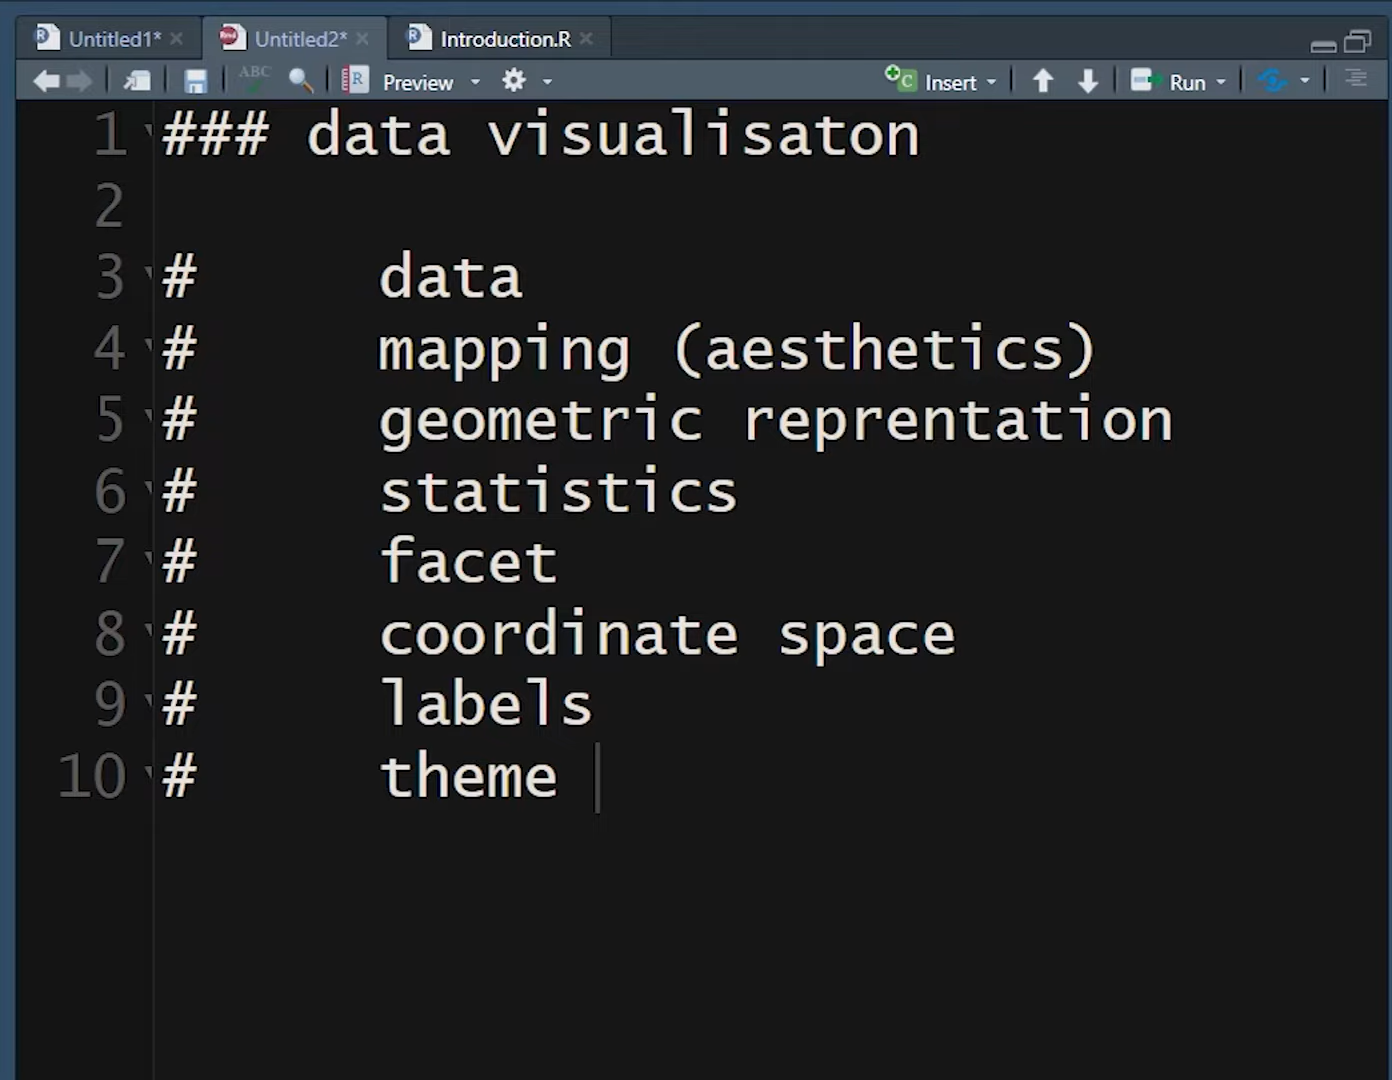
\includegraphics[scale = 0.15]{figure_1}
\end{figure}

\begin{knitrout}
\definecolor{shadecolor}{rgb}{0.969, 0.969, 0.969}\color{fgcolor}\begin{kframe}
\begin{alltt}
\hlcom{# install.packages('tidyverse')}

\hlkwd{library}\hlstd{(tidyverse)}
\end{alltt}


{\ttfamily\noindent\color{warningcolor}{\#\# Warning: package 'tidyverse' was built under R version 4.2.3}}

{\ttfamily\noindent\color{warningcolor}{\#\# Warning: package 'ggplot2' was built under R version 4.2.2}}

{\ttfamily\noindent\color{warningcolor}{\#\# Warning: package 'tibble' was built under R version 4.2.3}}

{\ttfamily\noindent\color{warningcolor}{\#\# Warning: package 'tidyr' was built under R version 4.2.3}}

{\ttfamily\noindent\color{warningcolor}{\#\# Warning: package 'readr' was built under R version 4.2.2}}

{\ttfamily\noindent\color{warningcolor}{\#\# Warning: package 'purrr' was built under R version 4.2.3}}

{\ttfamily\noindent\color{warningcolor}{\#\# Warning: package 'dplyr' was built under R version 4.2.3}}

{\ttfamily\noindent\color{warningcolor}{\#\# Warning: package 'stringr' was built under R version 4.2.3}}

{\ttfamily\noindent\color{warningcolor}{\#\# Warning: package 'forcats' was built under R version 4.2.2}}

{\ttfamily\noindent\color{warningcolor}{\#\# Warning: package 'lubridate' was built under R version 4.2.2}}

{\ttfamily\noindent\itshape\color{messagecolor}{\#\# -- Attaching core tidyverse packages ------------------------ tidyverse 2.0.0 --\\\#\# v dplyr \ \ \ \ 1.1.3 \ \ \ \ v readr \ \ \ \ 2.1.4\\\#\# v forcats \ \ 1.0.0 \ \ \ \ v stringr \ \ 1.5.0\\\#\# v ggplot2 \ \ 3.4.1 \ \ \ \ v tibble \ \ \ 3.2.1\\\#\# v lubridate 1.9.2 \ \ \ \ v tidyr \ \ \ \ 1.3.0\\\#\# v purrr \ \ \ \ 1.0.2 \ \ \ \ \\\#\# -- Conflicts ------------------------------------------ tidyverse\_conflicts() --\\\#\# x dplyr::filter() masks stats::filter()\\\#\# x dplyr::lag() \ \ \ masks stats::lag()\\\#\# i Use the conflicted package (<http://conflicted.r-lib.org/>) to force all conflicts to become errors}}\end{kframe}
\end{knitrout}

The function \textbf{data()} gives list of all data sets that are in-built in R.
\begin{knitrout}
\definecolor{shadecolor}{rgb}{0.969, 0.969, 0.969}\color{fgcolor}\begin{kframe}
\begin{alltt}
\hlkwd{data}\hlstd{()}
\end{alltt}
\end{kframe}
\end{knitrout}

We shall use \textbf{BOD} data set.
\begin{knitrout}
\definecolor{shadecolor}{rgb}{0.969, 0.969, 0.969}\color{fgcolor}\begin{kframe}
\begin{alltt}
\hlcom{# ?BOD}
\end{alltt}
\end{kframe}
\end{knitrout}

\begin{knitrout}
\definecolor{shadecolor}{rgb}{0.969, 0.969, 0.969}\color{fgcolor}\begin{kframe}
\begin{alltt}
\hlstd{BOD}
\end{alltt}
\begin{verbatim}
##   Time demand
## 1    1    8.3
## 2    2   10.3
## 3    3   19.0
## 4    4   16.0
## 5    5   15.6
## 6    7   19.8
\end{verbatim}
\end{kframe}
\end{knitrout}

\newpage

\begin{knitrout}
\definecolor{shadecolor}{rgb}{0.969, 0.969, 0.969}\color{fgcolor}\begin{kframe}
\begin{alltt}
\hlkwd{ggplot}\hlstd{(}\hlkwc{data} \hlstd{= BOD,} \hlkwc{mapping} \hlstd{=} \hlkwd{aes}\hlstd{(}\hlkwc{x} \hlstd{= Time,} \hlkwc{y} \hlstd{= demand))} \hlopt{+}
    \hlkwd{geom_point}\hlstd{(}\hlkwc{size} \hlstd{=} \hlnum{5}\hlstd{,} \hlkwc{colour} \hlstd{=} \hlstr{"red"}\hlstd{)} \hlopt{+} \hlkwd{geom_line}\hlstd{(}\hlkwc{color} \hlstd{=} \hlstr{"blue"}\hlstd{)}
\end{alltt}
\end{kframe}
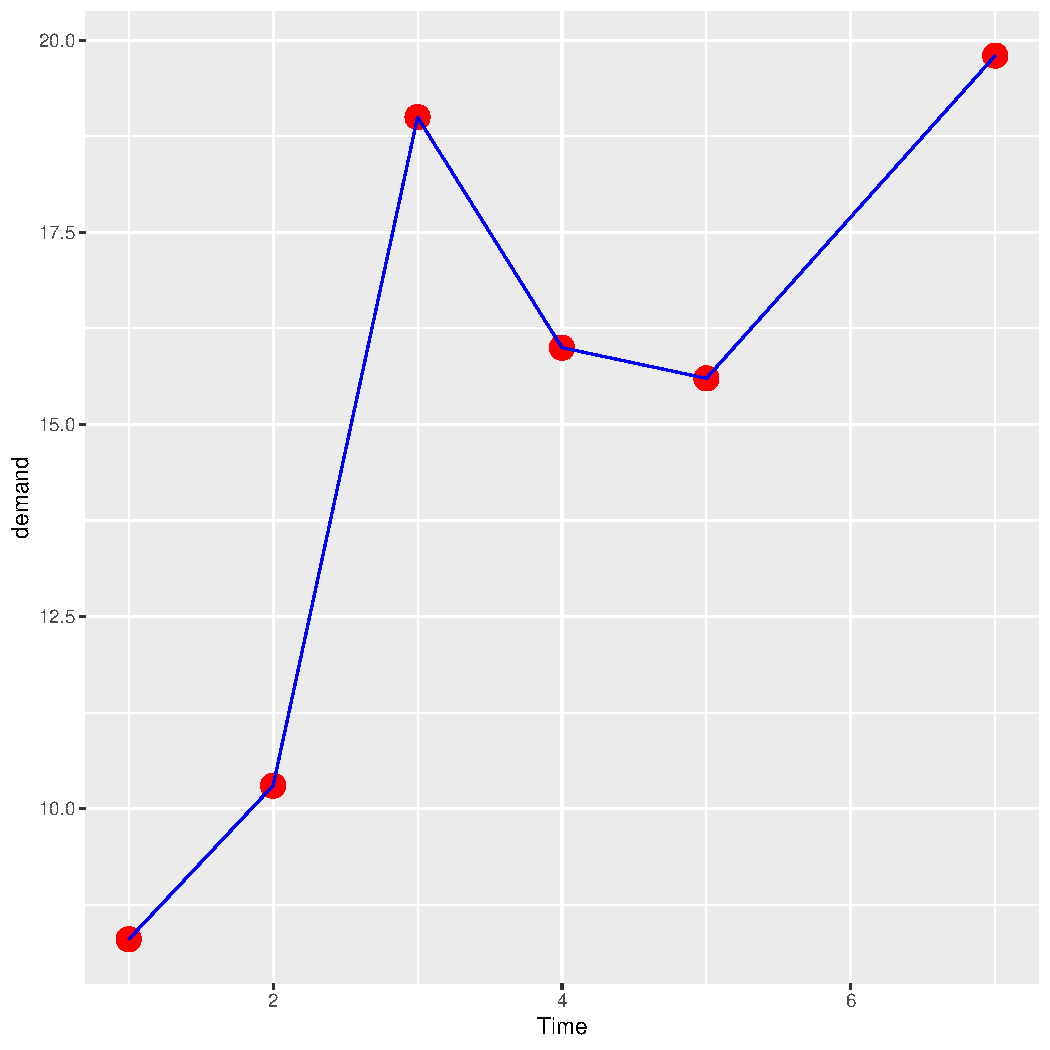
\includegraphics[width=\maxwidth]{figure/unnamed-chunk-5-1} 
\end{knitrout}

Now we shall use \textbf{CO2} data set.

\begin{knitrout}
\definecolor{shadecolor}{rgb}{0.969, 0.969, 0.969}\color{fgcolor}\begin{kframe}
\begin{alltt}
\hlkwd{view}\hlstd{(CO2)}
\end{alltt}
\end{kframe}
\end{knitrout}

\begin{knitrout}
\definecolor{shadecolor}{rgb}{0.969, 0.969, 0.969}\color{fgcolor}\begin{kframe}
\begin{alltt}
\hlcom{# ?CO2}
\end{alltt}
\end{kframe}
\end{knitrout}

\begin{knitrout}
\definecolor{shadecolor}{rgb}{0.969, 0.969, 0.969}\color{fgcolor}\begin{kframe}
\begin{alltt}
\hlkwd{names}\hlstd{(CO2)}
\end{alltt}
\begin{verbatim}
## [1] "Plant"     "Type"      "Treatment" "conc"      "uptake"
\end{verbatim}
\end{kframe}
\end{knitrout}

\textbf{\%$>$\%} is an operator in this context; often called pipe operator. The operand to its left is piped into as the first argument of the function ggplot(), which is to its right.

\newpage

\begin{knitrout}
\definecolor{shadecolor}{rgb}{0.969, 0.969, 0.969}\color{fgcolor}\begin{kframe}
\begin{alltt}
\hlstd{CO2} \hlopt
    \hlkwd{ggplot}\hlstd{(}\hlkwd{aes}\hlstd{(}\hlkwc{x} \hlstd{= conc,} \hlkwc{y} \hlstd{= uptake,} \hlkwc{colour} \hlstd{= Treatment))} \hlopt{+}
    \hlkwd{geom_point}\hlstd{()}
\end{alltt}
\end{kframe}
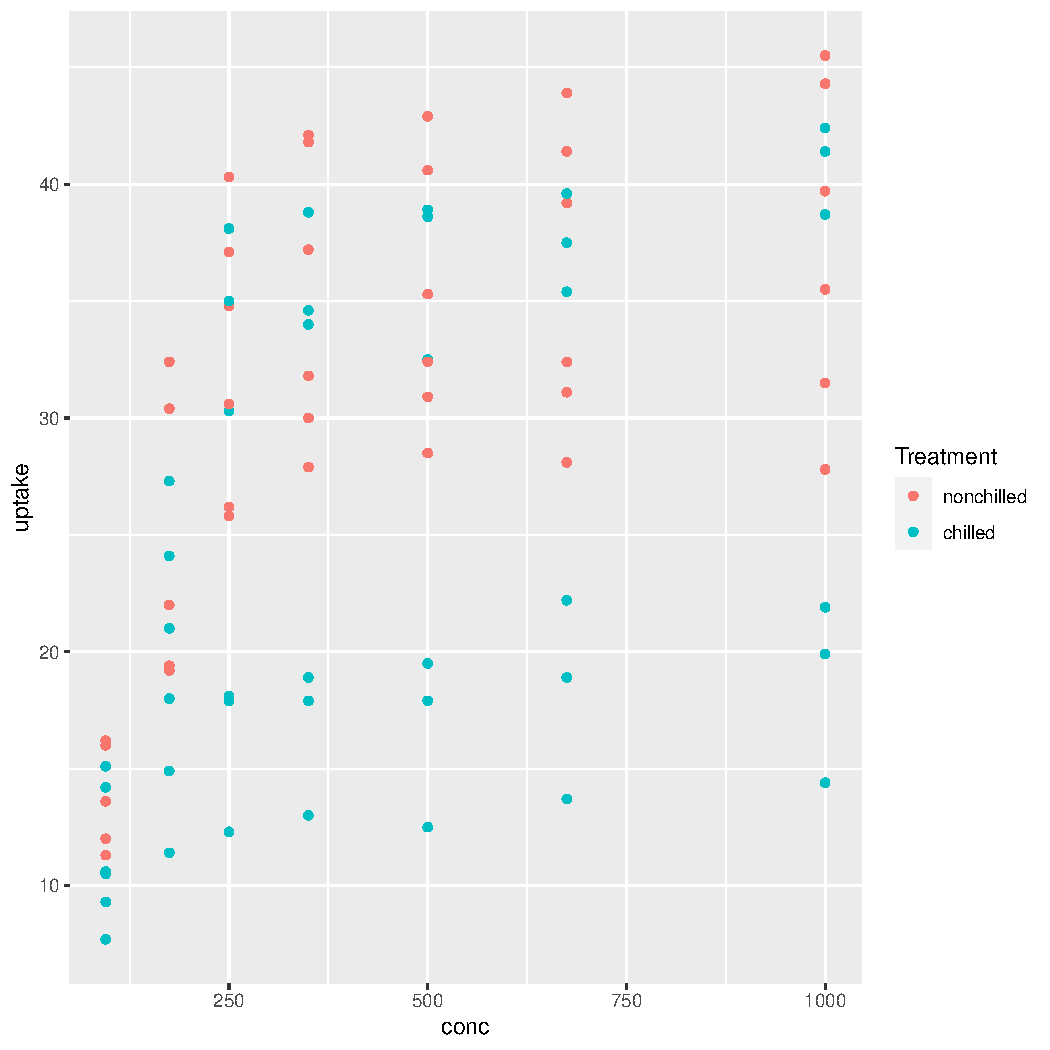
\includegraphics[width=\maxwidth]{figure/unnamed-chunk-9-1} 
\end{knitrout}

\newpage

\begin{knitrout}
\definecolor{shadecolor}{rgb}{0.969, 0.969, 0.969}\color{fgcolor}\begin{kframe}
\begin{alltt}
\hlstd{CO2} \hlopt
    \hlkwd{ggplot}\hlstd{(}\hlkwd{aes}\hlstd{(}\hlkwc{x} \hlstd{= conc,} \hlkwc{y} \hlstd{= uptake,} \hlkwc{color} \hlstd{= Treatment))} \hlopt{+}
    \hlkwd{geom_point}\hlstd{()} \hlopt{+} \hlkwd{labs}\hlstd{(}\hlkwc{title} \hlstd{=} \hlstr{"Concentartion of CO2"}\hlstd{)} \hlopt{+}
    \hlkwd{theme_bw}\hlstd{()}
\end{alltt}
\end{kframe}
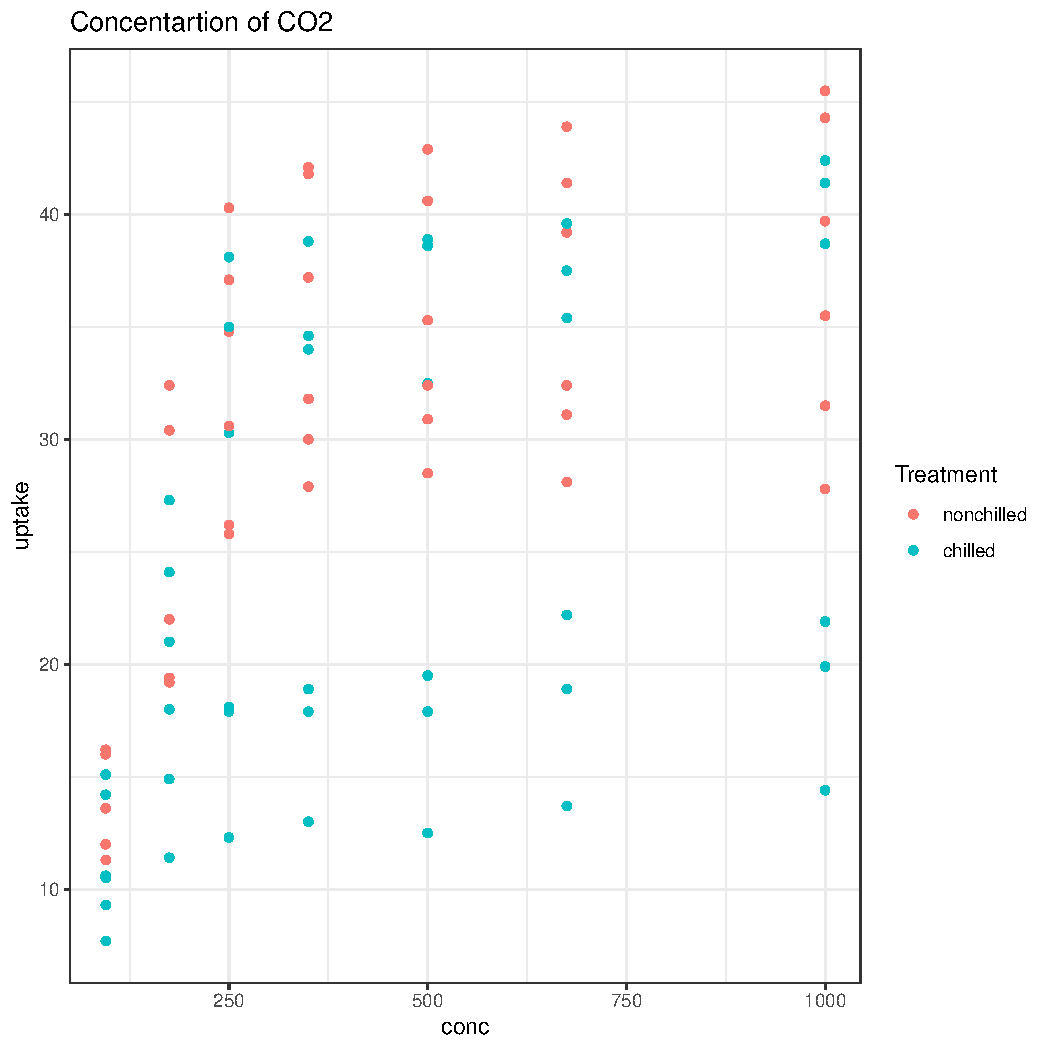
\includegraphics[width=\maxwidth]{figure/unnamed-chunk-10-1} 
\end{knitrout}

\newpage

\begin{knitrout}
\definecolor{shadecolor}{rgb}{0.969, 0.969, 0.969}\color{fgcolor}\begin{kframe}
\begin{alltt}
\hlstd{CO2} \hlopt
    \hlkwd{ggplot}\hlstd{(}\hlkwd{aes}\hlstd{(}\hlkwc{x} \hlstd{= Treatment,} \hlkwc{y} \hlstd{= uptake))} \hlopt{+} \hlkwd{geom_boxplot}\hlstd{()} \hlopt{+}
    \hlkwd{geom_point}\hlstd{(}\hlkwd{aes}\hlstd{(}\hlkwc{size} \hlstd{= conc,} \hlkwc{color} \hlstd{= Plant),} \hlkwc{alpha} \hlstd{=} \hlnum{0.5}\hlstd{)} \hlopt{+}
    \hlkwd{labs}\hlstd{(}\hlkwc{title} \hlstd{=} \hlstr{"Chilled vs Non-chilled"}\hlstd{)} \hlopt{+} \hlkwd{xlab}\hlstd{(}\hlstr{"Treatment"}\hlstd{)} \hlopt{+}
    \hlkwd{ylab}\hlstd{(}\hlstr{"Uptake"}\hlstd{)}
\end{alltt}
\end{kframe}
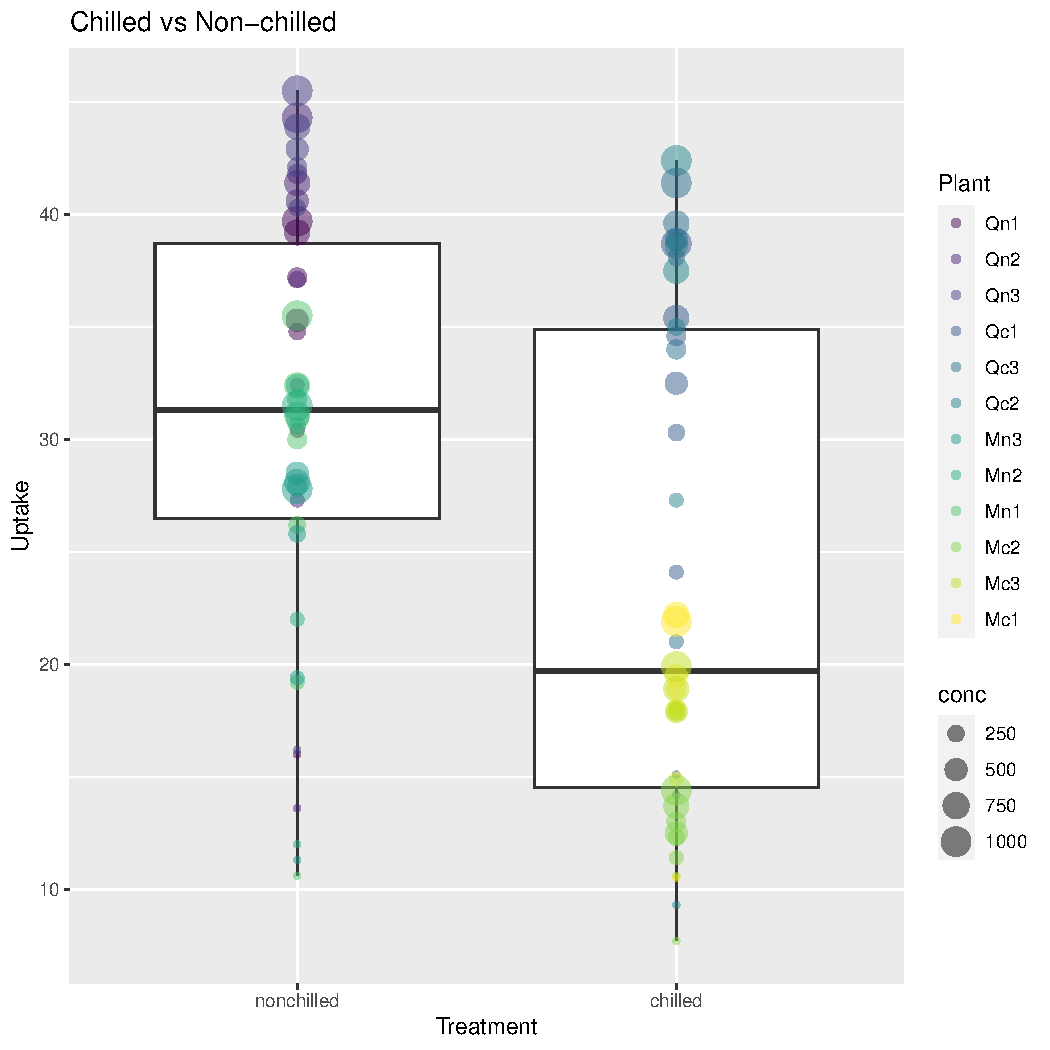
\includegraphics[width=\maxwidth]{figure/unnamed-chunk-11-1} 
\end{knitrout}

The argument \textit{alpha} stands for opacity. \\

The aesthetics of \textit{geom\_point()} will not influence others. But the aesthetics of \textit{ggplot()} will influence all others.

\newpage

\begin{knitrout}
\definecolor{shadecolor}{rgb}{0.969, 0.969, 0.969}\color{fgcolor}\begin{kframe}
\begin{alltt}
\hlstd{CO2} \hlopt
    \hlkwd{ggplot}\hlstd{(}\hlkwd{aes}\hlstd{(}\hlkwc{x} \hlstd{= Treatment,} \hlkwc{y} \hlstd{= uptake))} \hlopt{+} \hlkwd{geom_boxplot}\hlstd{()} \hlopt{+}
    \hlkwd{geom_point}\hlstd{(}\hlkwd{aes}\hlstd{(}\hlkwc{size} \hlstd{= conc,} \hlkwc{color} \hlstd{= Plant),} \hlkwc{alpha} \hlstd{=} \hlnum{0.5}\hlstd{)} \hlopt{+}
    \hlkwd{coord_flip}\hlstd{()}
\end{alltt}
\end{kframe}
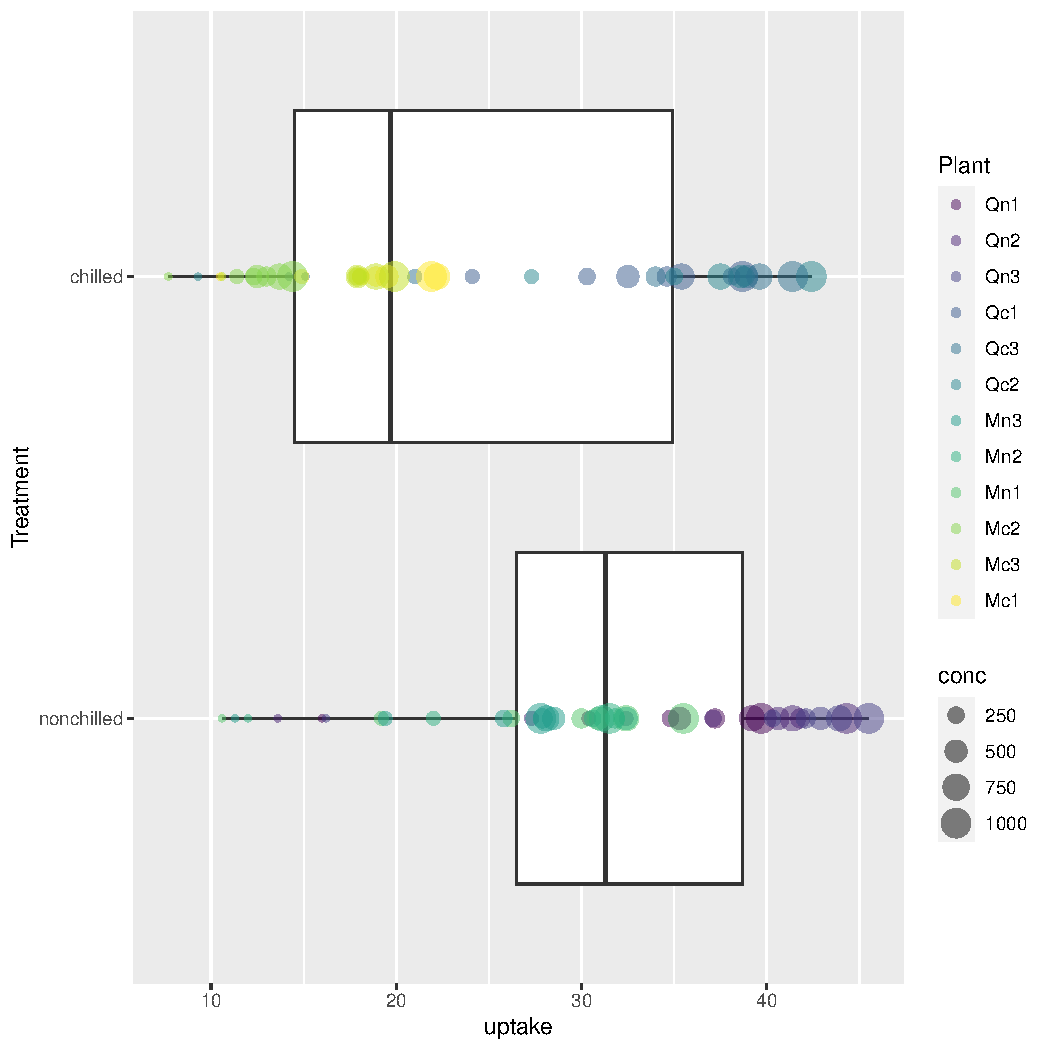
\includegraphics[width=\maxwidth]{figure/unnamed-chunk-12-1} 
\end{knitrout}

Now we shall use \textbf{msleep} data set.
\begin{knitrout}
\definecolor{shadecolor}{rgb}{0.969, 0.969, 0.969}\color{fgcolor}\begin{kframe}
\begin{alltt}
\hlcom{# ?msleep}
\end{alltt}
\end{kframe}
\end{knitrout}

\begin{knitrout}
\definecolor{shadecolor}{rgb}{0.969, 0.969, 0.969}\color{fgcolor}\begin{kframe}
\begin{alltt}
\hlkwd{names}\hlstd{(msleep)}
\end{alltt}
\begin{verbatim}
##  [1] "name"         "genus"        "vore"         "order"        "conservation"
##  [6] "sleep_total"  "sleep_rem"    "sleep_cycle"  "awake"        "brainwt"     
## [11] "bodywt"
\end{verbatim}
\end{kframe}
\end{knitrout}

\begin{knitrout}
\definecolor{shadecolor}{rgb}{0.969, 0.969, 0.969}\color{fgcolor}\begin{kframe}
\begin{alltt}
\hlkwd{view}\hlstd{(msleep)}
\end{alltt}
\end{kframe}
\end{knitrout}

\section*{Barplot}

\begin{knitrout}
\definecolor{shadecolor}{rgb}{0.969, 0.969, 0.969}\color{fgcolor}\begin{kframe}
\begin{alltt}
\hlstd{msleep} \hlopt
    \hlkwd{drop_na}\hlstd{(vore)} \hlopt
    \hlkwd{ggplot}\hlstd{(}\hlkwd{aes}\hlstd{(}\hlkwc{x} \hlstd{= vore))} \hlopt{+} \hlkwd{geom_bar}\hlstd{(}\hlkwc{fill} \hlstd{=} \hlstr{"#0A96F7"}\hlstd{,}
    \hlkwc{color} \hlstd{=} \hlstr{"black"}\hlstd{,} \hlkwc{linewidth} \hlstd{=} \hlnum{1}\hlstd{)} \hlopt{+} \hlkwd{labs}\hlstd{(}\hlkwc{x} \hlstd{=} \hlstr{"Vore"}\hlstd{,}
    \hlkwc{y} \hlstd{=} \hlstr{"Frequency"}\hlstd{,} \hlkwc{title} \hlstd{=} \hlstr{"Barplot of different vores"}\hlstd{)}
\end{alltt}
\end{kframe}
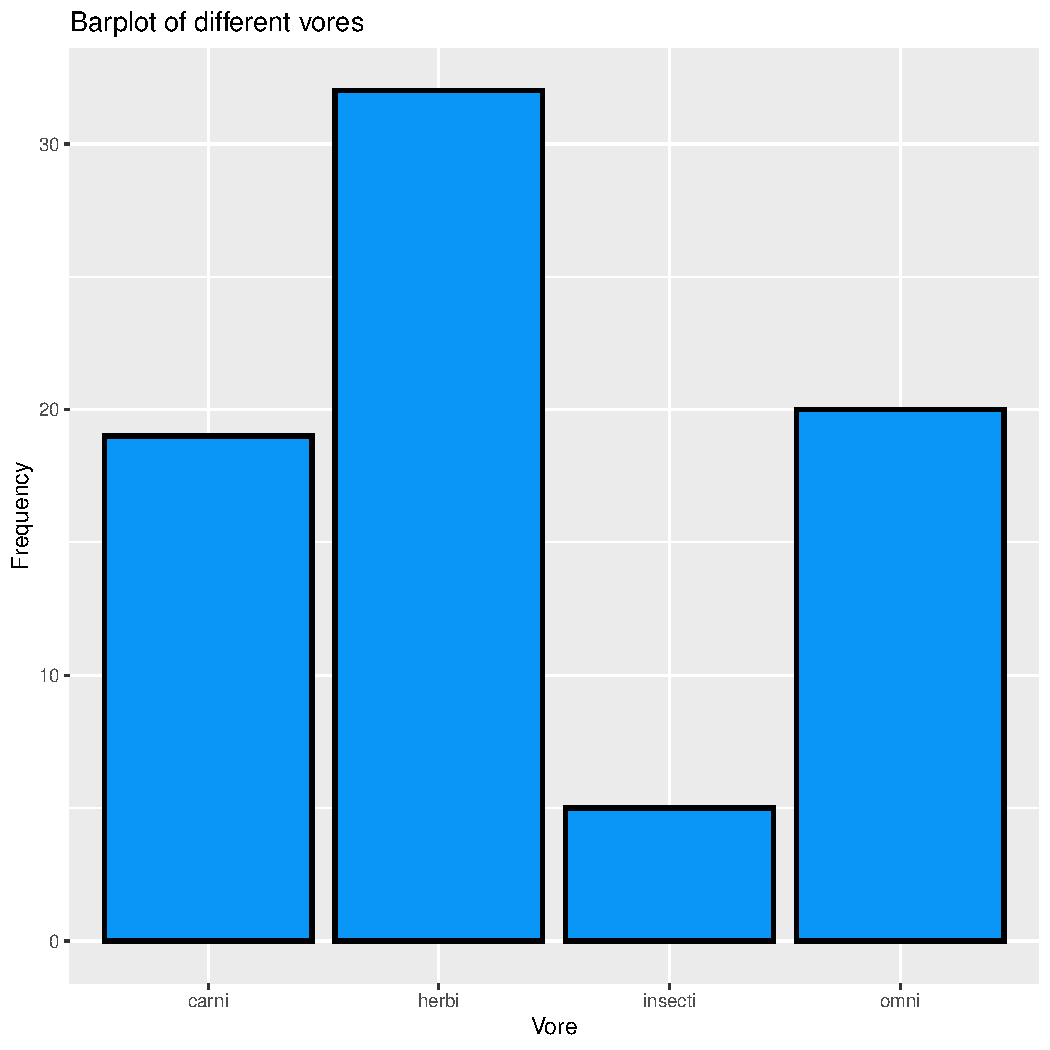
\includegraphics[width=\maxwidth]{figure/unnamed-chunk-16-1} 
\end{knitrout}

\textbf{drop\_na(vore)} drops the \textit{NA} values from the variable \textit{vore} and pipes the filtered data set to ggplot.

\newpage

\begin{knitrout}
\definecolor{shadecolor}{rgb}{0.969, 0.969, 0.969}\color{fgcolor}\begin{kframe}
\begin{alltt}
\hlstd{msleep} \hlopt
    \hlkwd{drop_na}\hlstd{(vore)} \hlopt
    \hlkwd{ggplot}\hlstd{(}\hlkwd{aes}\hlstd{(}\hlkwc{x} \hlstd{= vore))} \hlopt{+} \hlkwd{geom_bar}\hlstd{(}\hlkwc{fill} \hlstd{=} \hlstr{"#BE0AF7"}\hlstd{,}
    \hlkwc{color} \hlstd{=} \hlstr{"black"}\hlstd{,} \hlkwc{linewidth} \hlstd{=} \hlnum{1}\hlstd{)} \hlopt{+} \hlkwd{coord_flip}\hlstd{()} \hlopt{+}
    \hlkwd{labs}\hlstd{(}\hlkwc{x} \hlstd{=} \hlstr{"Vore"}\hlstd{,} \hlkwc{y} \hlstd{=} \hlstr{"Frequency"}\hlstd{,} \hlkwc{title} \hlstd{=} \hlstr{"Barplot of different vores"}\hlstd{)}
\end{alltt}
\end{kframe}
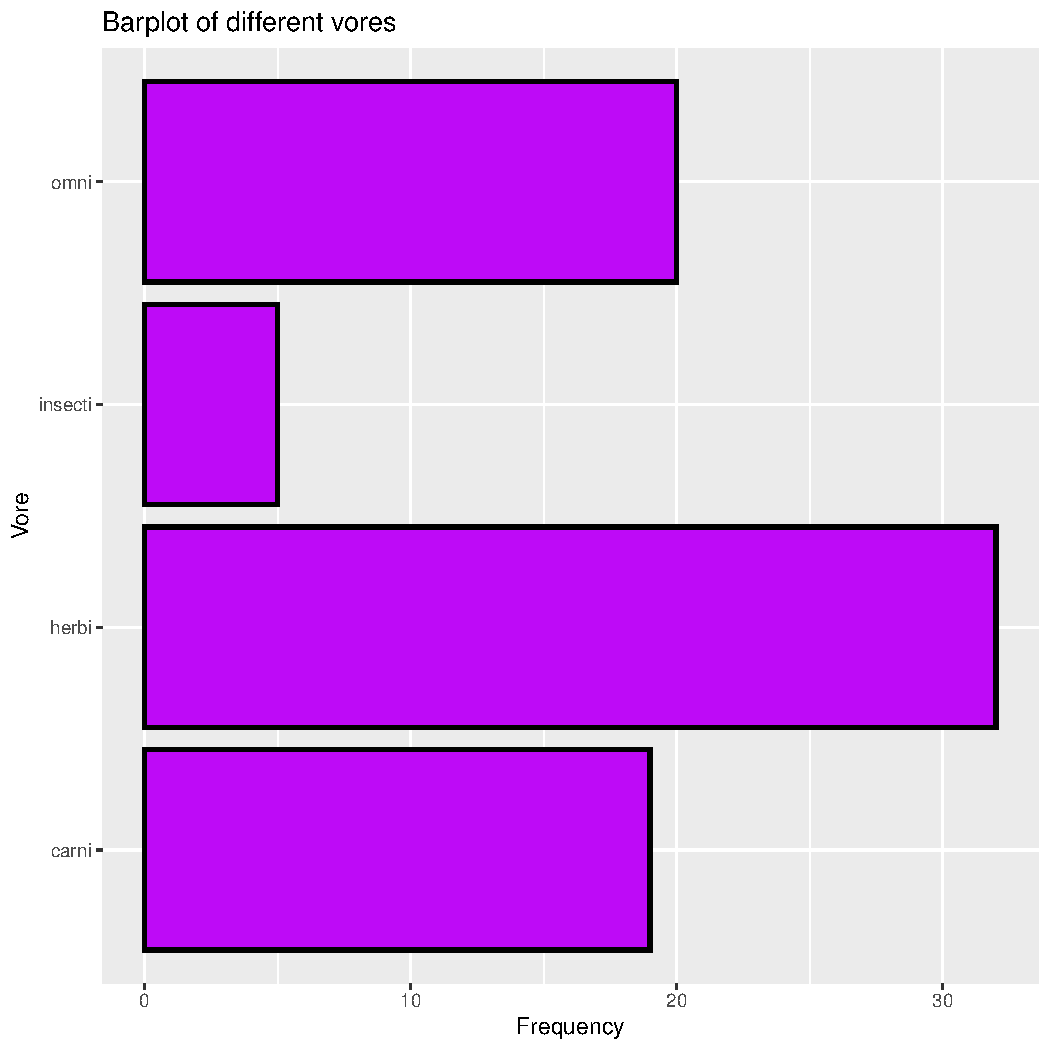
\includegraphics[width=\maxwidth]{figure/unnamed-chunk-17-1} 
\end{knitrout}

\newpage

\begin{knitrout}
\definecolor{shadecolor}{rgb}{0.969, 0.969, 0.969}\color{fgcolor}\begin{kframe}
\begin{alltt}
\hlstd{msleep} \hlopt
    \hlkwd{drop_na}\hlstd{(vore)} \hlopt
    \hlkwd{ggplot}\hlstd{(}\hlkwd{aes}\hlstd{(}\hlkwc{x} \hlstd{=} \hlkwd{fct_infreq}\hlstd{(vore)))} \hlopt{+} \hlkwd{geom_bar}\hlstd{(}\hlkwc{fill} \hlstd{=} \hlstr{"#FB069E"}\hlstd{,}
    \hlkwc{color} \hlstd{=} \hlstr{"black"}\hlstd{,} \hlkwc{linewidth} \hlstd{=} \hlnum{1}\hlstd{)} \hlopt{+} \hlkwd{labs}\hlstd{(}\hlkwc{x} \hlstd{=} \hlstr{"Vore"}\hlstd{,}
    \hlkwc{y} \hlstd{=} \hlstr{"Frequency"}\hlstd{,} \hlkwc{title} \hlstd{=} \hlstr{"Barplot of different vores"}\hlstd{)}
\end{alltt}
\end{kframe}
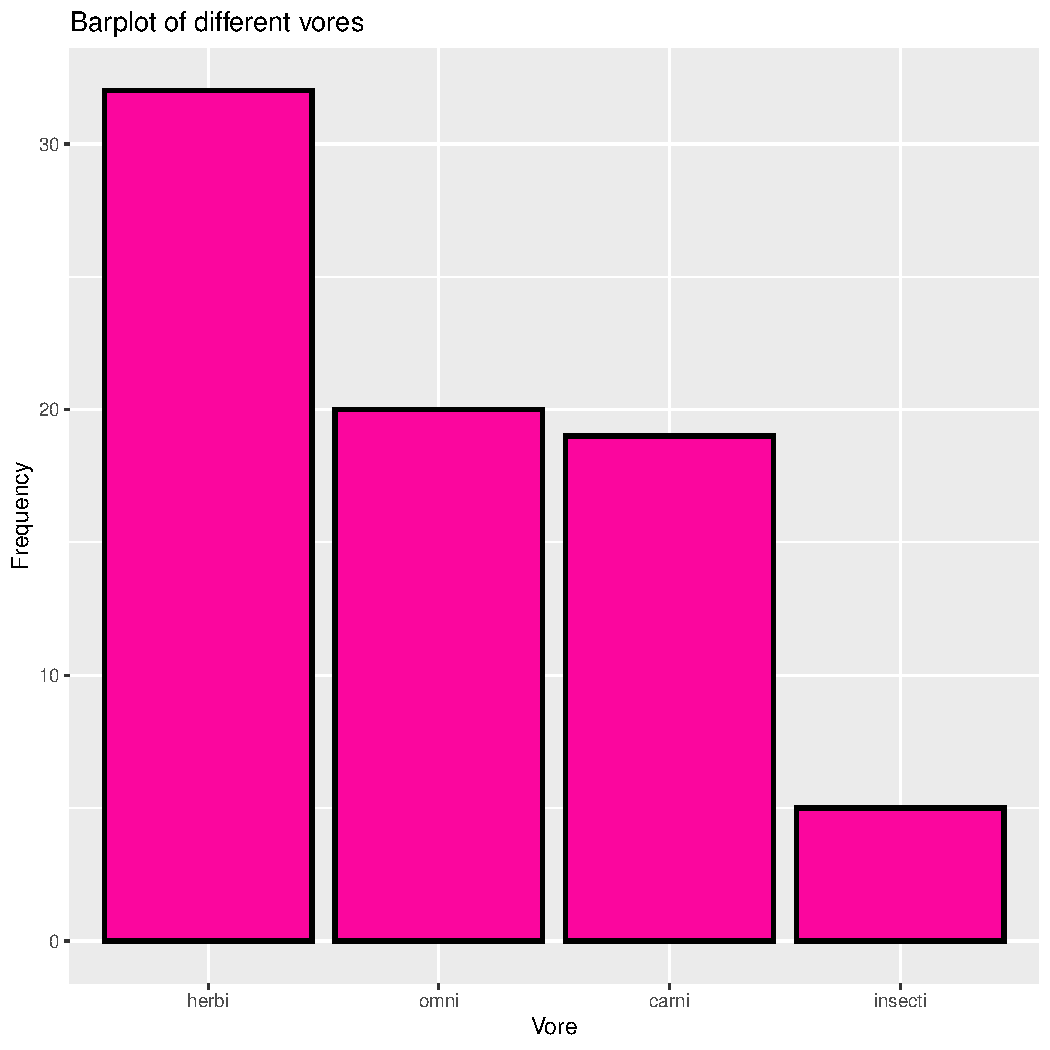
\includegraphics[width=\maxwidth]{figure/unnamed-chunk-18-1} 
\end{knitrout}

\newpage

\begin{knitrout}
\definecolor{shadecolor}{rgb}{0.969, 0.969, 0.969}\color{fgcolor}\begin{kframe}
\begin{alltt}
\hlstd{random_binomial_numbers} \hlkwb{<-} \hlkwd{rbinom}\hlstd{(}\hlkwc{n} \hlstd{=} \hlnum{20000}\hlstd{,} \hlkwc{size} \hlstd{=} \hlnum{10}\hlstd{,}
    \hlkwc{prob} \hlstd{=} \hlnum{0.5}\hlstd{)}

\hlstd{random_binomial_numbers} \hlkwb{<-} \hlkwd{data.frame}\hlstd{(random_binomial_numbers)}

\hlkwd{ggplot}\hlstd{(random_binomial_numbers,} \hlkwd{aes}\hlstd{(}\hlkwc{x} \hlstd{= random_binomial_numbers))} \hlopt{+}
    \hlkwd{geom_bar}\hlstd{(}\hlkwc{fill} \hlstd{=} \hlstr{"#FB8C06"}\hlstd{,} \hlkwc{color} \hlstd{=} \hlstr{"black"}\hlstd{,} \hlkwc{linewidth} \hlstd{=} \hlnum{1}\hlstd{)} \hlopt{+}
    \hlkwd{labs}\hlstd{(}\hlkwc{x} \hlstd{=} \hlstr{"Numbers"}\hlstd{,} \hlkwc{y} \hlstd{=} \hlstr{"Frequency"}\hlstd{,} \hlkwc{title} \hlstd{=} \hlstr{"Barplot of Binomial(10, 0.5)"}\hlstd{)}
\end{alltt}
\end{kframe}
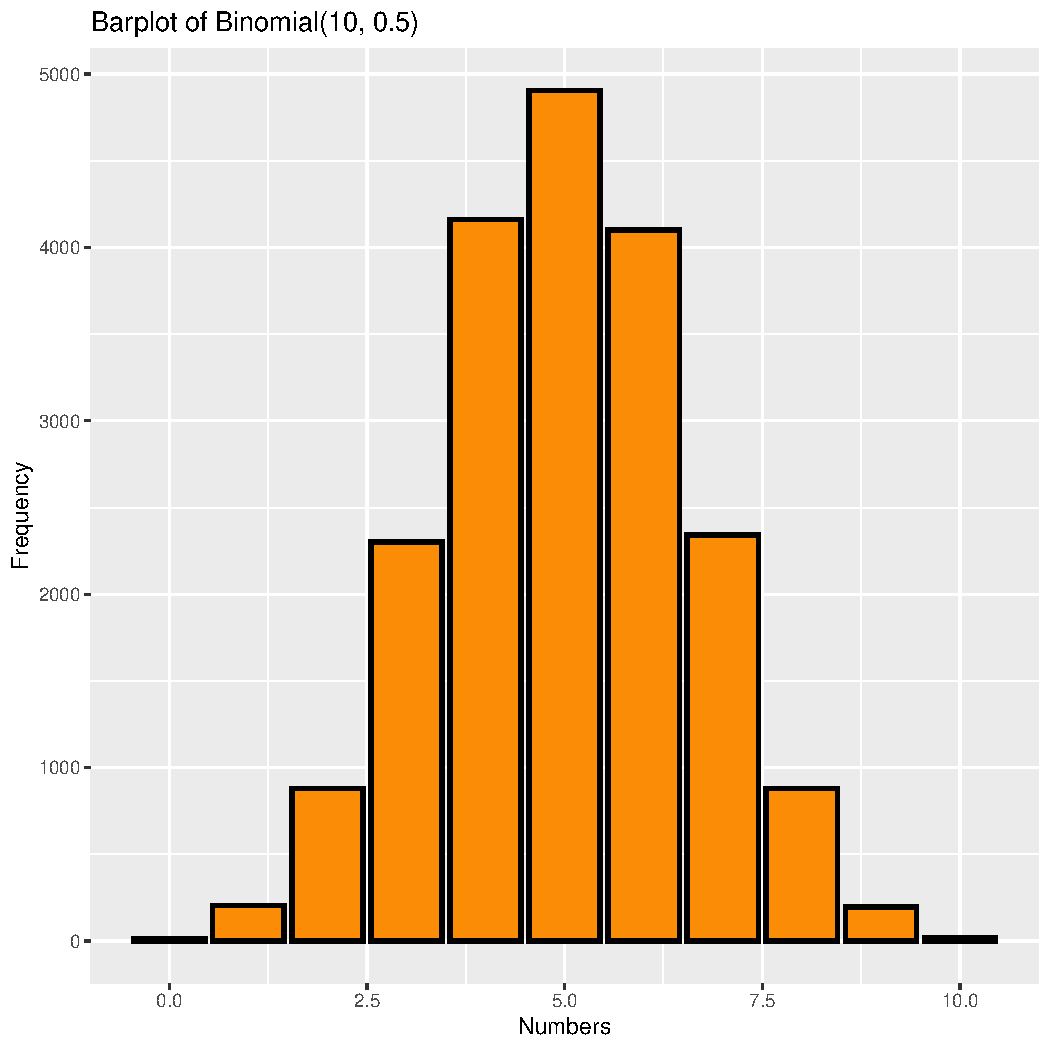
\includegraphics[width=\maxwidth]{figure/unnamed-chunk-19-1} 
\end{knitrout}

\newpage

\begin{knitrout}
\definecolor{shadecolor}{rgb}{0.969, 0.969, 0.969}\color{fgcolor}\begin{kframe}
\begin{alltt}
\hlstd{random_poisson_numbers} \hlkwb{<-} \hlkwd{rpois}\hlstd{(}\hlkwc{n} \hlstd{=} \hlnum{20000}\hlstd{,} \hlkwc{lambda} \hlstd{=} \hlnum{2}\hlstd{)}

\hlstd{random_poisson_numbers} \hlkwb{<-} \hlkwd{data.frame}\hlstd{(random_poisson_numbers)}

\hlkwd{ggplot}\hlstd{(random_poisson_numbers,} \hlkwd{aes}\hlstd{(}\hlkwc{x} \hlstd{= random_poisson_numbers))} \hlopt{+}
    \hlkwd{geom_bar}\hlstd{(}\hlkwc{fill} \hlstd{=} \hlstr{"#FB8C06"}\hlstd{,} \hlkwc{color} \hlstd{=} \hlstr{"black"}\hlstd{,} \hlkwc{linewidth} \hlstd{=} \hlnum{1}\hlstd{)} \hlopt{+}
    \hlkwd{labs}\hlstd{(}\hlkwc{x} \hlstd{=} \hlstr{"Numbers"}\hlstd{,} \hlkwc{y} \hlstd{=} \hlstr{"Frequency"}\hlstd{,} \hlkwc{title} \hlstd{=} \hlstr{"Barplot of Poisson(2)"}\hlstd{)}
\end{alltt}
\end{kframe}
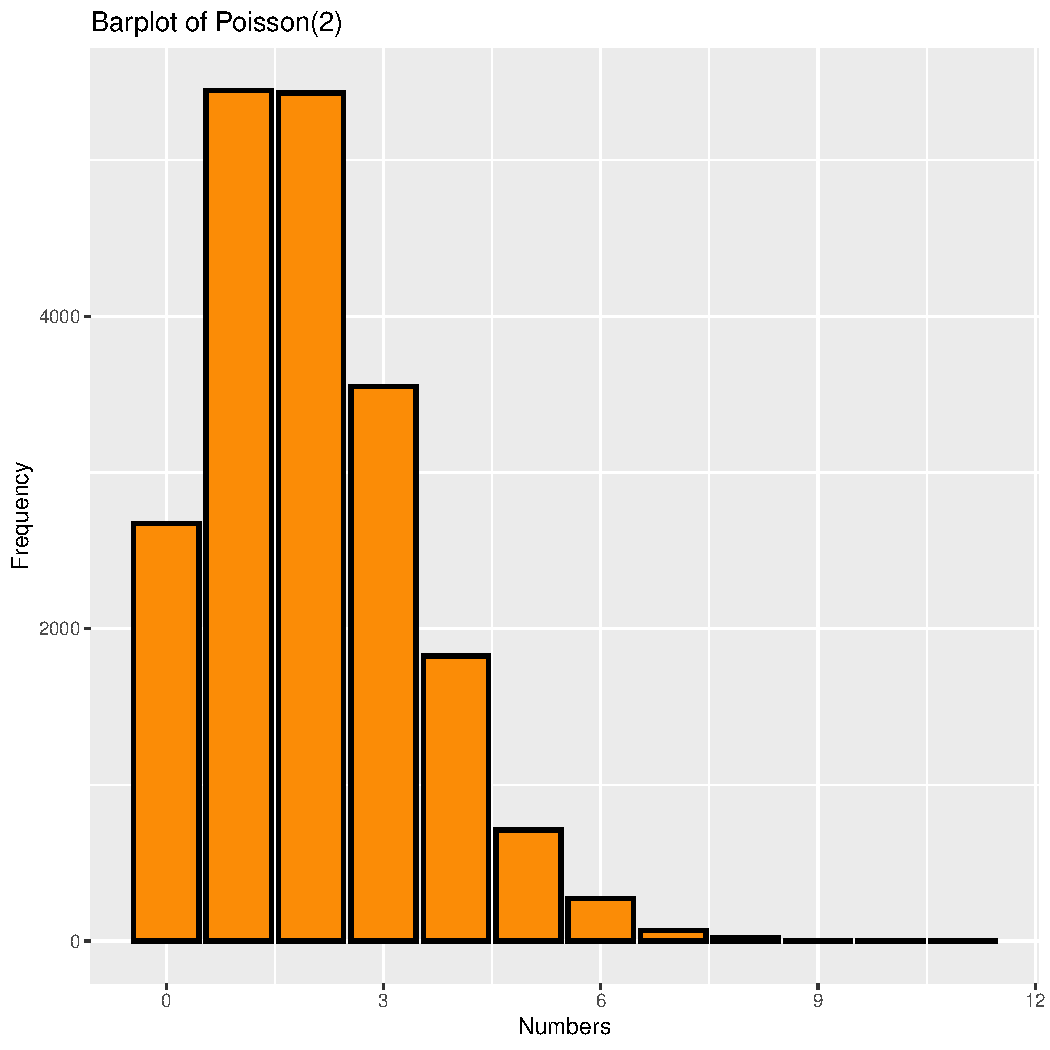
\includegraphics[width=\maxwidth]{figure/unnamed-chunk-20-1} 
\end{knitrout}

\newpage

\section*{Histogram}

\begin{knitrout}
\definecolor{shadecolor}{rgb}{0.969, 0.969, 0.969}\color{fgcolor}\begin{kframe}
\begin{alltt}
\hlstd{random_normal_numbers} \hlkwb{<-} \hlkwd{rnorm}\hlstd{(}\hlkwc{n} \hlstd{=} \hlnum{20000}\hlstd{,} \hlkwc{mean} \hlstd{=} \hlnum{0}\hlstd{,}
    \hlkwc{sd} \hlstd{=} \hlnum{1}\hlstd{)}

\hlstd{random_normal_numbers} \hlkwb{<-} \hlkwd{data.frame}\hlstd{(random_normal_numbers)}

\hlstd{random_normal_numbers} \hlopt
    \hlkwd{ggplot}\hlstd{(}\hlkwd{aes}\hlstd{(}\hlkwc{x} \hlstd{= random_normal_numbers))} \hlopt{+} \hlkwd{geom_histogram}\hlstd{(}\hlkwc{binwidth} \hlstd{=} \hlnum{0.35}\hlstd{,}
    \hlkwc{fill} \hlstd{=} \hlstr{"#0FD8F0"}\hlstd{,} \hlkwc{color} \hlstd{=} \hlstr{"black"}\hlstd{,} \hlkwc{linewidth} \hlstd{=} \hlnum{1}\hlstd{)} \hlopt{+}
    \hlkwd{labs}\hlstd{(}\hlkwc{x} \hlstd{=} \hlstr{"Numbers"}\hlstd{,} \hlkwc{y} \hlstd{=} \hlstr{"Frequency"}\hlstd{,} \hlkwc{title} \hlstd{=} \hlstr{"Histogram of N(0, 1)"}\hlstd{)}
\end{alltt}
\end{kframe}
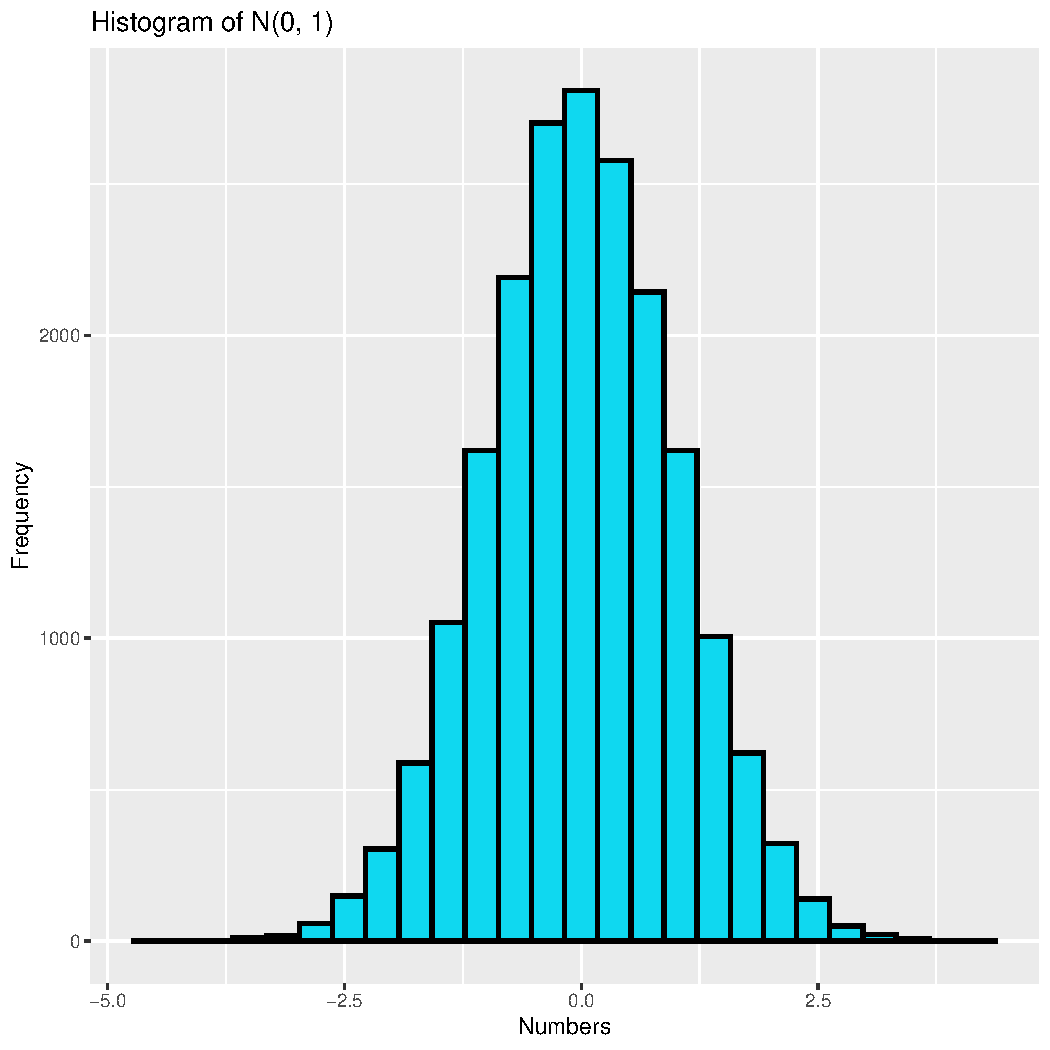
\includegraphics[width=\maxwidth]{figure/unnamed-chunk-21-1} 
\end{knitrout}

$\bullet$ Observe that, the parameter \textbf{binwidth} controls the number of bins in the histogram. The bigger the binwidth, the less the number of bins and vice versa.

Now we shall use \textbf{iris} data set.

\begin{knitrout}
\definecolor{shadecolor}{rgb}{0.969, 0.969, 0.969}\color{fgcolor}\begin{kframe}
\begin{alltt}
\hlkwd{View}\hlstd{(iris)}
\end{alltt}
\end{kframe}
\end{knitrout}

\begin{knitrout}
\definecolor{shadecolor}{rgb}{0.969, 0.969, 0.969}\color{fgcolor}\begin{kframe}
\begin{alltt}
\hlkwd{names}\hlstd{(iris)}
\end{alltt}
\begin{verbatim}
## [1] "Sepal.Length" "Sepal.Width"  "Petal.Length" "Petal.Width"  "Species"
\end{verbatim}
\end{kframe}
\end{knitrout}

\newpage

\begin{knitrout}
\definecolor{shadecolor}{rgb}{0.969, 0.969, 0.969}\color{fgcolor}\begin{kframe}
\begin{alltt}
\hlstd{iris} \hlopt
    \hlkwd{ggplot}\hlstd{(}\hlkwd{aes}\hlstd{(}\hlkwc{x} \hlstd{= Sepal.Length,} \hlkwc{y} \hlstd{= Petal.Length,}
        \hlkwc{color} \hlstd{= Species))} \hlopt{+} \hlkwd{geom_point}\hlstd{()} \hlopt{+} \hlkwd{labs}\hlstd{(}\hlkwc{x} \hlstd{=} \hlstr{"Sepal Length"}\hlstd{,}
    \hlkwc{y} \hlstd{=} \hlstr{"Petal Length"}\hlstd{,} \hlkwc{title} \hlstd{=} \hlstr{"Sepal Length vs Petal Length"}\hlstd{)}
\end{alltt}
\end{kframe}
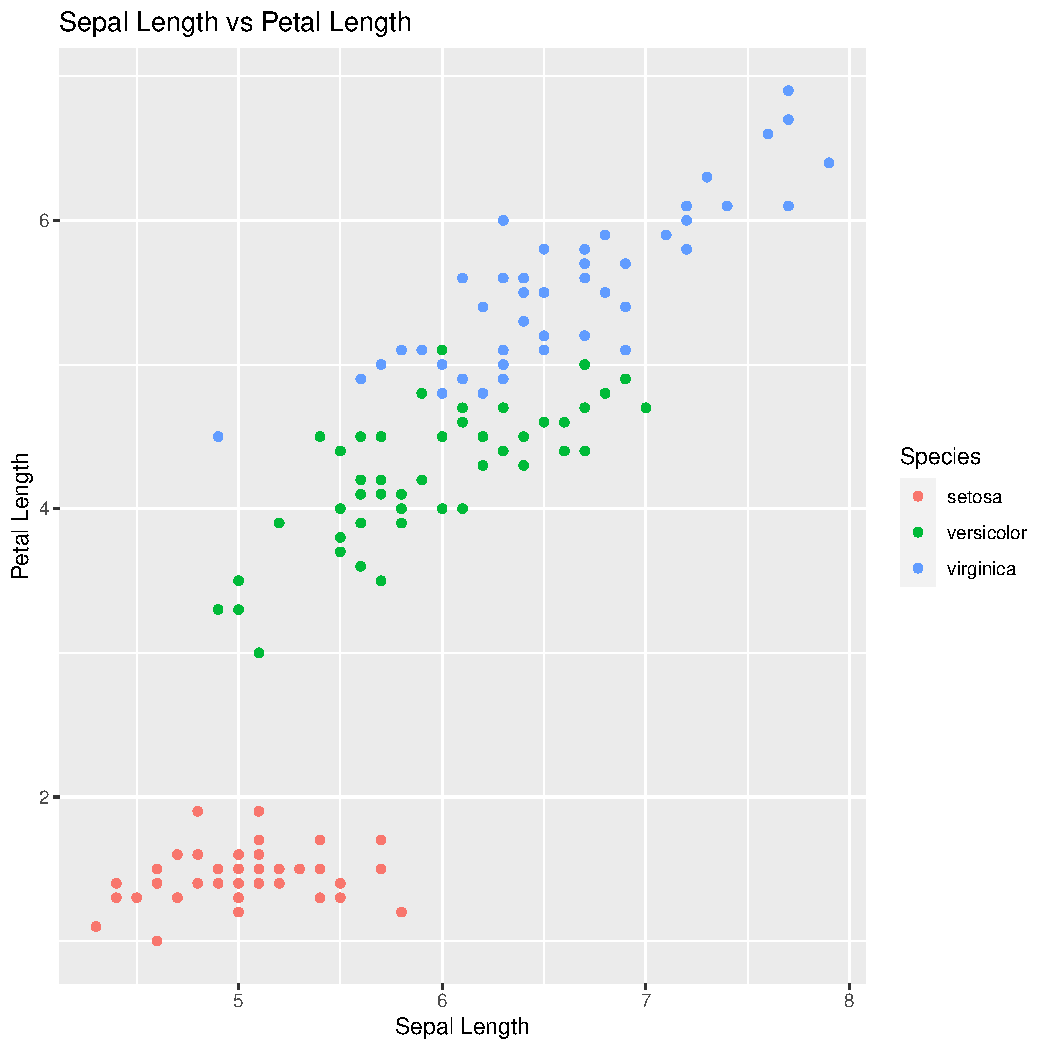
\includegraphics[width=\maxwidth]{figure/unnamed-chunk-24-1} 
\end{knitrout}

\newpage

\begin{knitrout}
\definecolor{shadecolor}{rgb}{0.969, 0.969, 0.969}\color{fgcolor}\begin{kframe}
\begin{alltt}
\hlstd{iris} \hlopt
    \hlkwd{filter}\hlstd{(Species} \hlopt{==} \hlstr{"versicolor"}\hlstd{)} \hlopt
    \hlkwd{ggplot}\hlstd{(}\hlkwd{aes}\hlstd{(}\hlkwc{x} \hlstd{= Sepal.Length,} \hlkwc{y} \hlstd{= Petal.Length))} \hlopt{+}
    \hlkwd{geom_point}\hlstd{(}\hlkwc{col} \hlstd{=} \hlstr{"#0FF020"}\hlstd{)} \hlopt{+} \hlkwd{labs}\hlstd{(}\hlkwc{x} \hlstd{=} \hlstr{"Sepal Length"}\hlstd{,}
    \hlkwc{y} \hlstd{=} \hlstr{"Petal Length"}\hlstd{,} \hlkwc{title} \hlstd{=} \hlstr{"Sepal Length vs Petal Length of Versicolor"}\hlstd{)}
\end{alltt}
\end{kframe}
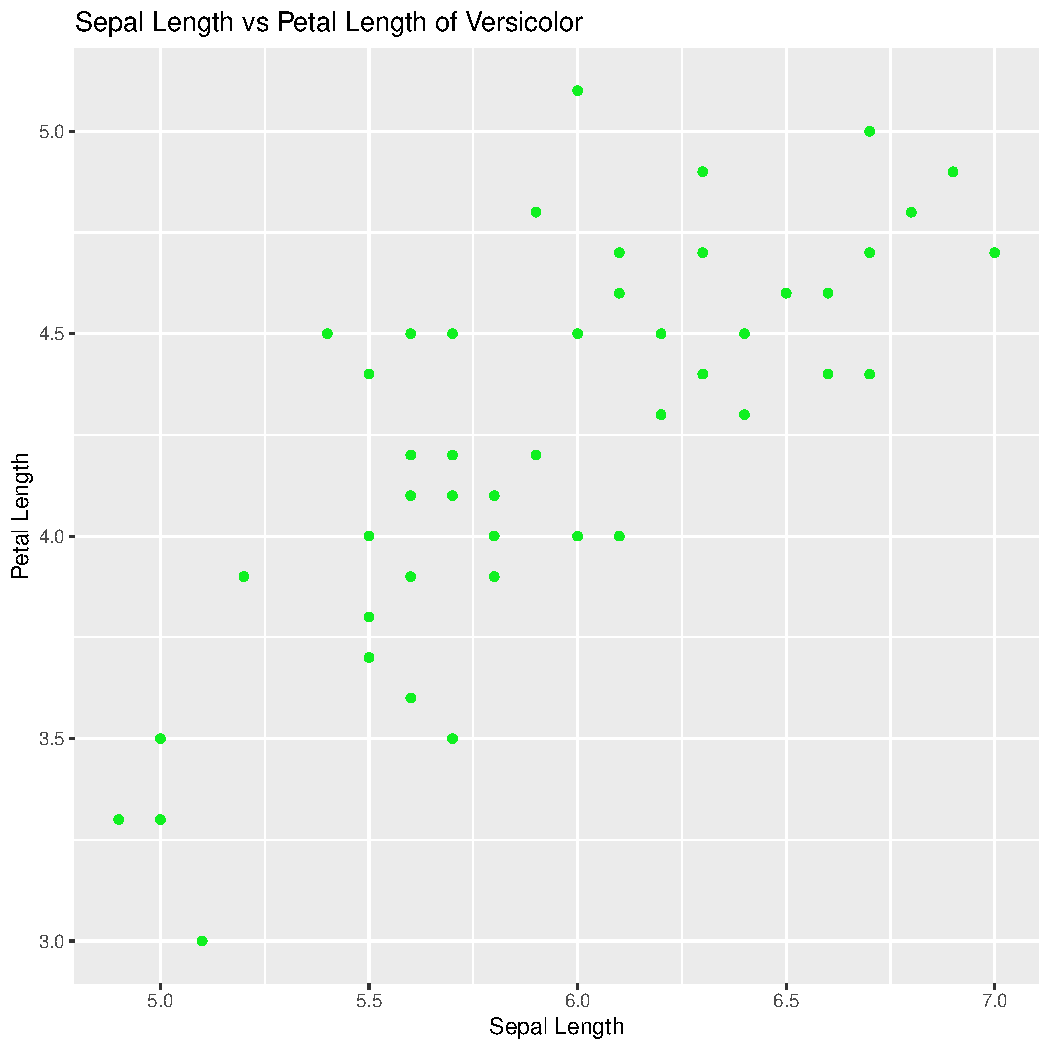
\includegraphics[width=\maxwidth]{figure/unnamed-chunk-25-1} 
\end{knitrout}

\newpage

\begin{knitrout}
\definecolor{shadecolor}{rgb}{0.969, 0.969, 0.969}\color{fgcolor}\begin{kframe}
\begin{alltt}
\hlstd{iris} \hlopt
    \hlkwd{ggplot}\hlstd{(}\hlkwd{aes}\hlstd{(}\hlkwc{x} \hlstd{= Sepal.Width,} \hlkwc{y} \hlstd{= Petal.Width,} \hlkwc{color} \hlstd{= Species))} \hlopt{+}
    \hlkwd{geom_point}\hlstd{()} \hlopt{+} \hlkwd{labs}\hlstd{(}\hlkwc{x} \hlstd{=} \hlstr{"Sepal Width"}\hlstd{,} \hlkwc{y} \hlstd{=} \hlstr{"Petal Width"}\hlstd{,}
    \hlkwc{title} \hlstd{=} \hlstr{"Sepal Width vs Petal Width"}\hlstd{)}
\end{alltt}
\end{kframe}
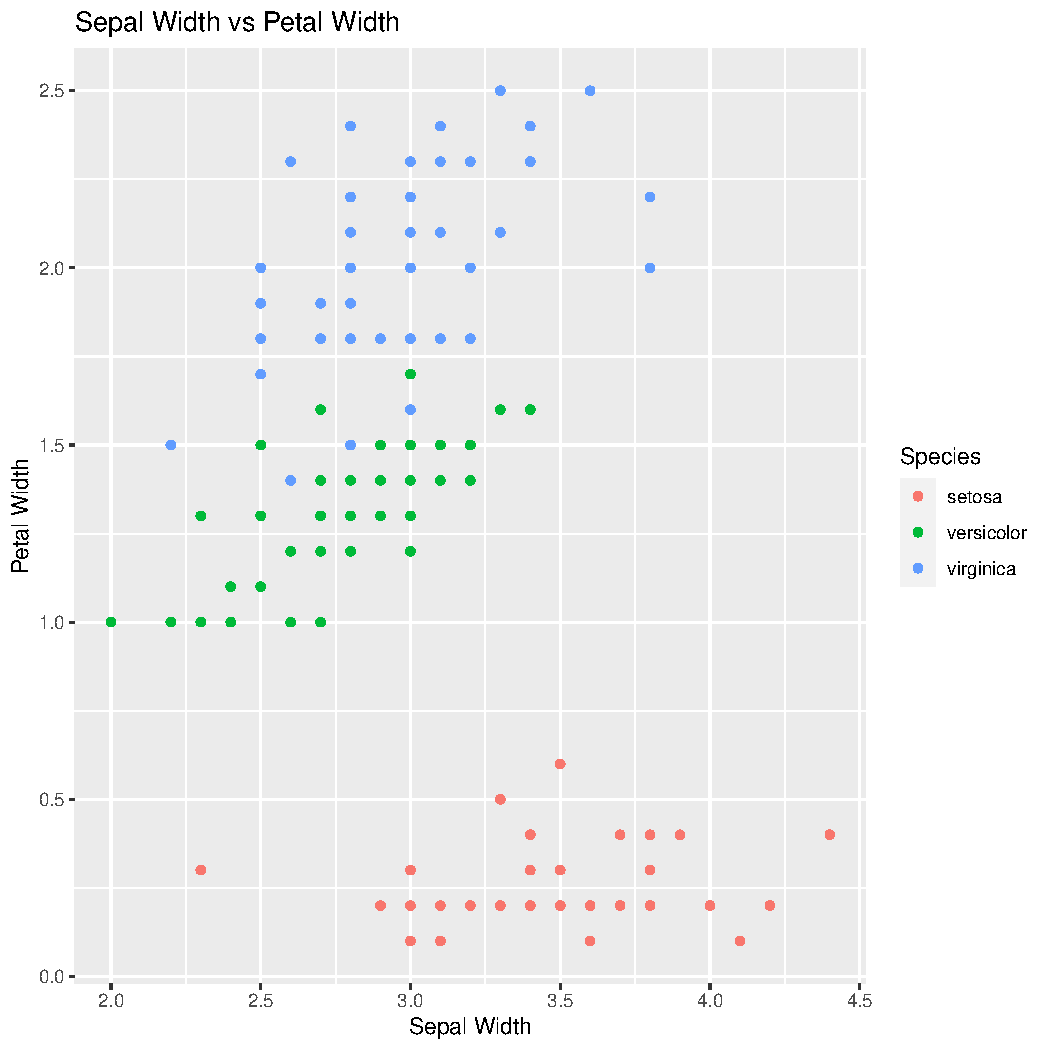
\includegraphics[width=\maxwidth]{figure/unnamed-chunk-26-1} 
\end{knitrout}

\newpage

\begin{knitrout}
\definecolor{shadecolor}{rgb}{0.969, 0.969, 0.969}\color{fgcolor}\begin{kframe}
\begin{alltt}
\hlstd{deepak_ntr_data} \hlkwb{<-} \hlkwd{read.csv}\hlstd{(}\hlstr{"DEEPAKNTR-21-09-2023-to-02-10-2023.csv"}\hlstd{)}
\end{alltt}
\end{kframe}
\end{knitrout}

\begin{knitrout}
\definecolor{shadecolor}{rgb}{0.969, 0.969, 0.969}\color{fgcolor}\begin{kframe}
\begin{alltt}
\hlkwd{names}\hlstd{(deepak_ntr_data)}
\end{alltt}
\begin{verbatim}
##  [1] "Date"         "series"       "OPEN"         "HIGH"         "LOW"         
##  [6] "PREV..CLOSE"  "ltp"          "close"        "vwap"         "X52W.H"      
## [11] "X52W.L"       "VOLUME"       "VALUE"        "No.of.trades"
\end{verbatim}
\end{kframe}
\end{knitrout}

\begin{knitrout}
\definecolor{shadecolor}{rgb}{0.969, 0.969, 0.969}\color{fgcolor}\begin{kframe}
\begin{alltt}
\hlkwd{str}\hlstd{(deepak_ntr_data)}
\end{alltt}
\begin{verbatim}
## 'data.frame':	7 obs. of  14 variables:
##  $ Date        : chr  "29-09-2023" "28-09-2023" "27-09-2023" "26-09-2023" ...
##  $ series      : chr  "EQ" "EQ" "EQ" "EQ" ...
##  $ OPEN        : num  2101 2142 2115 2148 2127 ...
##  $ HIGH        : num  2140 2156 2150 2154 2157 ...
##  $ LOW         : num  2091 2082 2100 2100 2121 ...
##  $ PREV..CLOSE : num  2100 2142 2108 2138 2128 ...
##  $ ltp         : num  2119 2109 2140 2114 2138 ...
##  $ close       : num  2120 2100 2142 2108 2138 ...
##  $ vwap        : num  2119 2118 2131 2127 2144 ...
##  $ X52W.H      : num  2373 2373 2373 2373 2373 ...
##  $ X52W.L      : num  1730 1730 1730 1730 1730 1730 1730
##  $ VOLUME      : num  155386 230858 249896 263970 219732 ...
##  $ VALUE       : num  3.29e+08 4.89e+08 5.33e+08 5.61e+08 4.71e+08 ...
##  $ No.of.trades: num  12906 19540 20854 20503 21331 ...
\end{verbatim}
\end{kframe}
\end{knitrout}


\begin{knitrout}
\definecolor{shadecolor}{rgb}{0.969, 0.969, 0.969}\color{fgcolor}\begin{kframe}
\begin{alltt}
\hlkwd{sapply}\hlstd{(deepak_ntr_data, class)}
\end{alltt}
\begin{verbatim}
##         Date       series         OPEN         HIGH          LOW  PREV..CLOSE 
##  "character"  "character"    "numeric"    "numeric"    "numeric"    "numeric" 
##          ltp        close         vwap       X52W.H       X52W.L       VOLUME 
##    "numeric"    "numeric"    "numeric"    "numeric"    "numeric"    "numeric" 
##        VALUE No.of.trades 
##    "numeric"    "numeric"
\end{verbatim}
\end{kframe}
\end{knitrout}

We see that the class of \textit{Date} is \textit{chr}. We shall change it.

\begin{knitrout}
\definecolor{shadecolor}{rgb}{0.969, 0.969, 0.969}\color{fgcolor}\begin{kframe}
\begin{alltt}
\hlstd{deepak_ntr_data}\hlopt{$}\hlstd{Date} \hlkwb{<-} \hlkwd{as.POSIXct}\hlstd{(deepak_ntr_data}\hlopt{$}\hlstd{Date)}
\end{alltt}
\end{kframe}
\end{knitrout}

We want to do a line graph of the closing price. The most recent observation is at first in the data set.

\newpage

\begin{knitrout}
\definecolor{shadecolor}{rgb}{0.969, 0.969, 0.969}\color{fgcolor}\begin{kframe}
\begin{alltt}
\hlstd{deepak_ntr_data} \hlopt
    \hlkwd{ggplot}\hlstd{(}\hlkwd{aes}\hlstd{(}\hlkwc{x} \hlstd{=} \hlkwd{rev}\hlstd{(Date),} \hlkwc{y} \hlstd{=} \hlkwd{rev}\hlstd{(close)))} \hlopt{+} \hlkwd{geom_point}\hlstd{()} \hlopt{+}
    \hlkwd{geom_line}\hlstd{()} \hlopt{+} \hlkwd{geom_ribbon}\hlstd{(}\hlkwd{aes}\hlstd{(}\hlkwc{ymin} \hlstd{=} \hlkwd{min}\hlstd{(close)} \hlopt{-}
    \hlnum{10}\hlstd{,} \hlkwc{ymax} \hlstd{=} \hlkwd{rev}\hlstd{(close)),} \hlkwc{fill} \hlstd{=} \hlstr{"#EE6573"}\hlstd{)} \hlopt{+} \hlkwd{labs}\hlstd{(}\hlkwc{x} \hlstd{=} \hlstr{"Date"}\hlstd{,}
    \hlkwc{y} \hlstd{=} \hlstr{"Closing Price"}\hlstd{,} \hlkwc{title} \hlstd{=} \hlstr{"Closing Price of D-NTR - 21-29 Sep"}\hlstd{)}
\end{alltt}
\end{kframe}
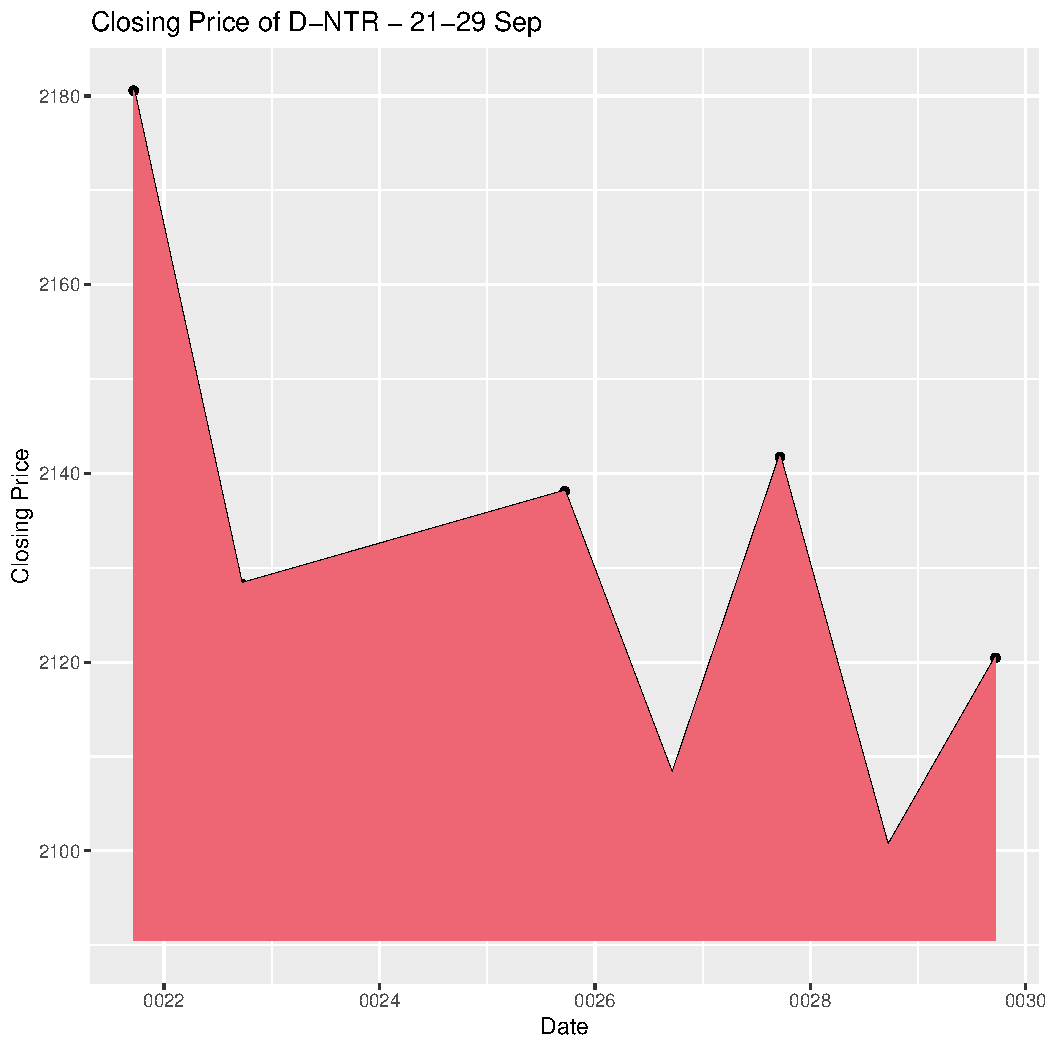
\includegraphics[width=\maxwidth]{figure/unnamed-chunk-32-1} 
\end{knitrout}



\end{document}
